After the system requirement document has been aproved, the system context diagram could be made (see figure \ref*{fig:sys-context-top}).
The block called "Audio DSP" is the heart of the system.
This block represents the controller and thus the FPGA core.
This system context design diagram fulfills all the requirements, including the should and could haves.
Therefore the Audio-DSP has four analogue inputs, one USB input and six analogue outputs.
The input select line is for selecting what line input you want on input channel 1 and 2.
The user can either select a RCA or 6.35mm jack input on input channel 1 and 2.

With a user interface the user is able to configure the effect parameters, equalizer settings and volume of each channel.
The user is also able to rearrange the position of effects in the effects loop per channel.

\begin{figure}[h]
    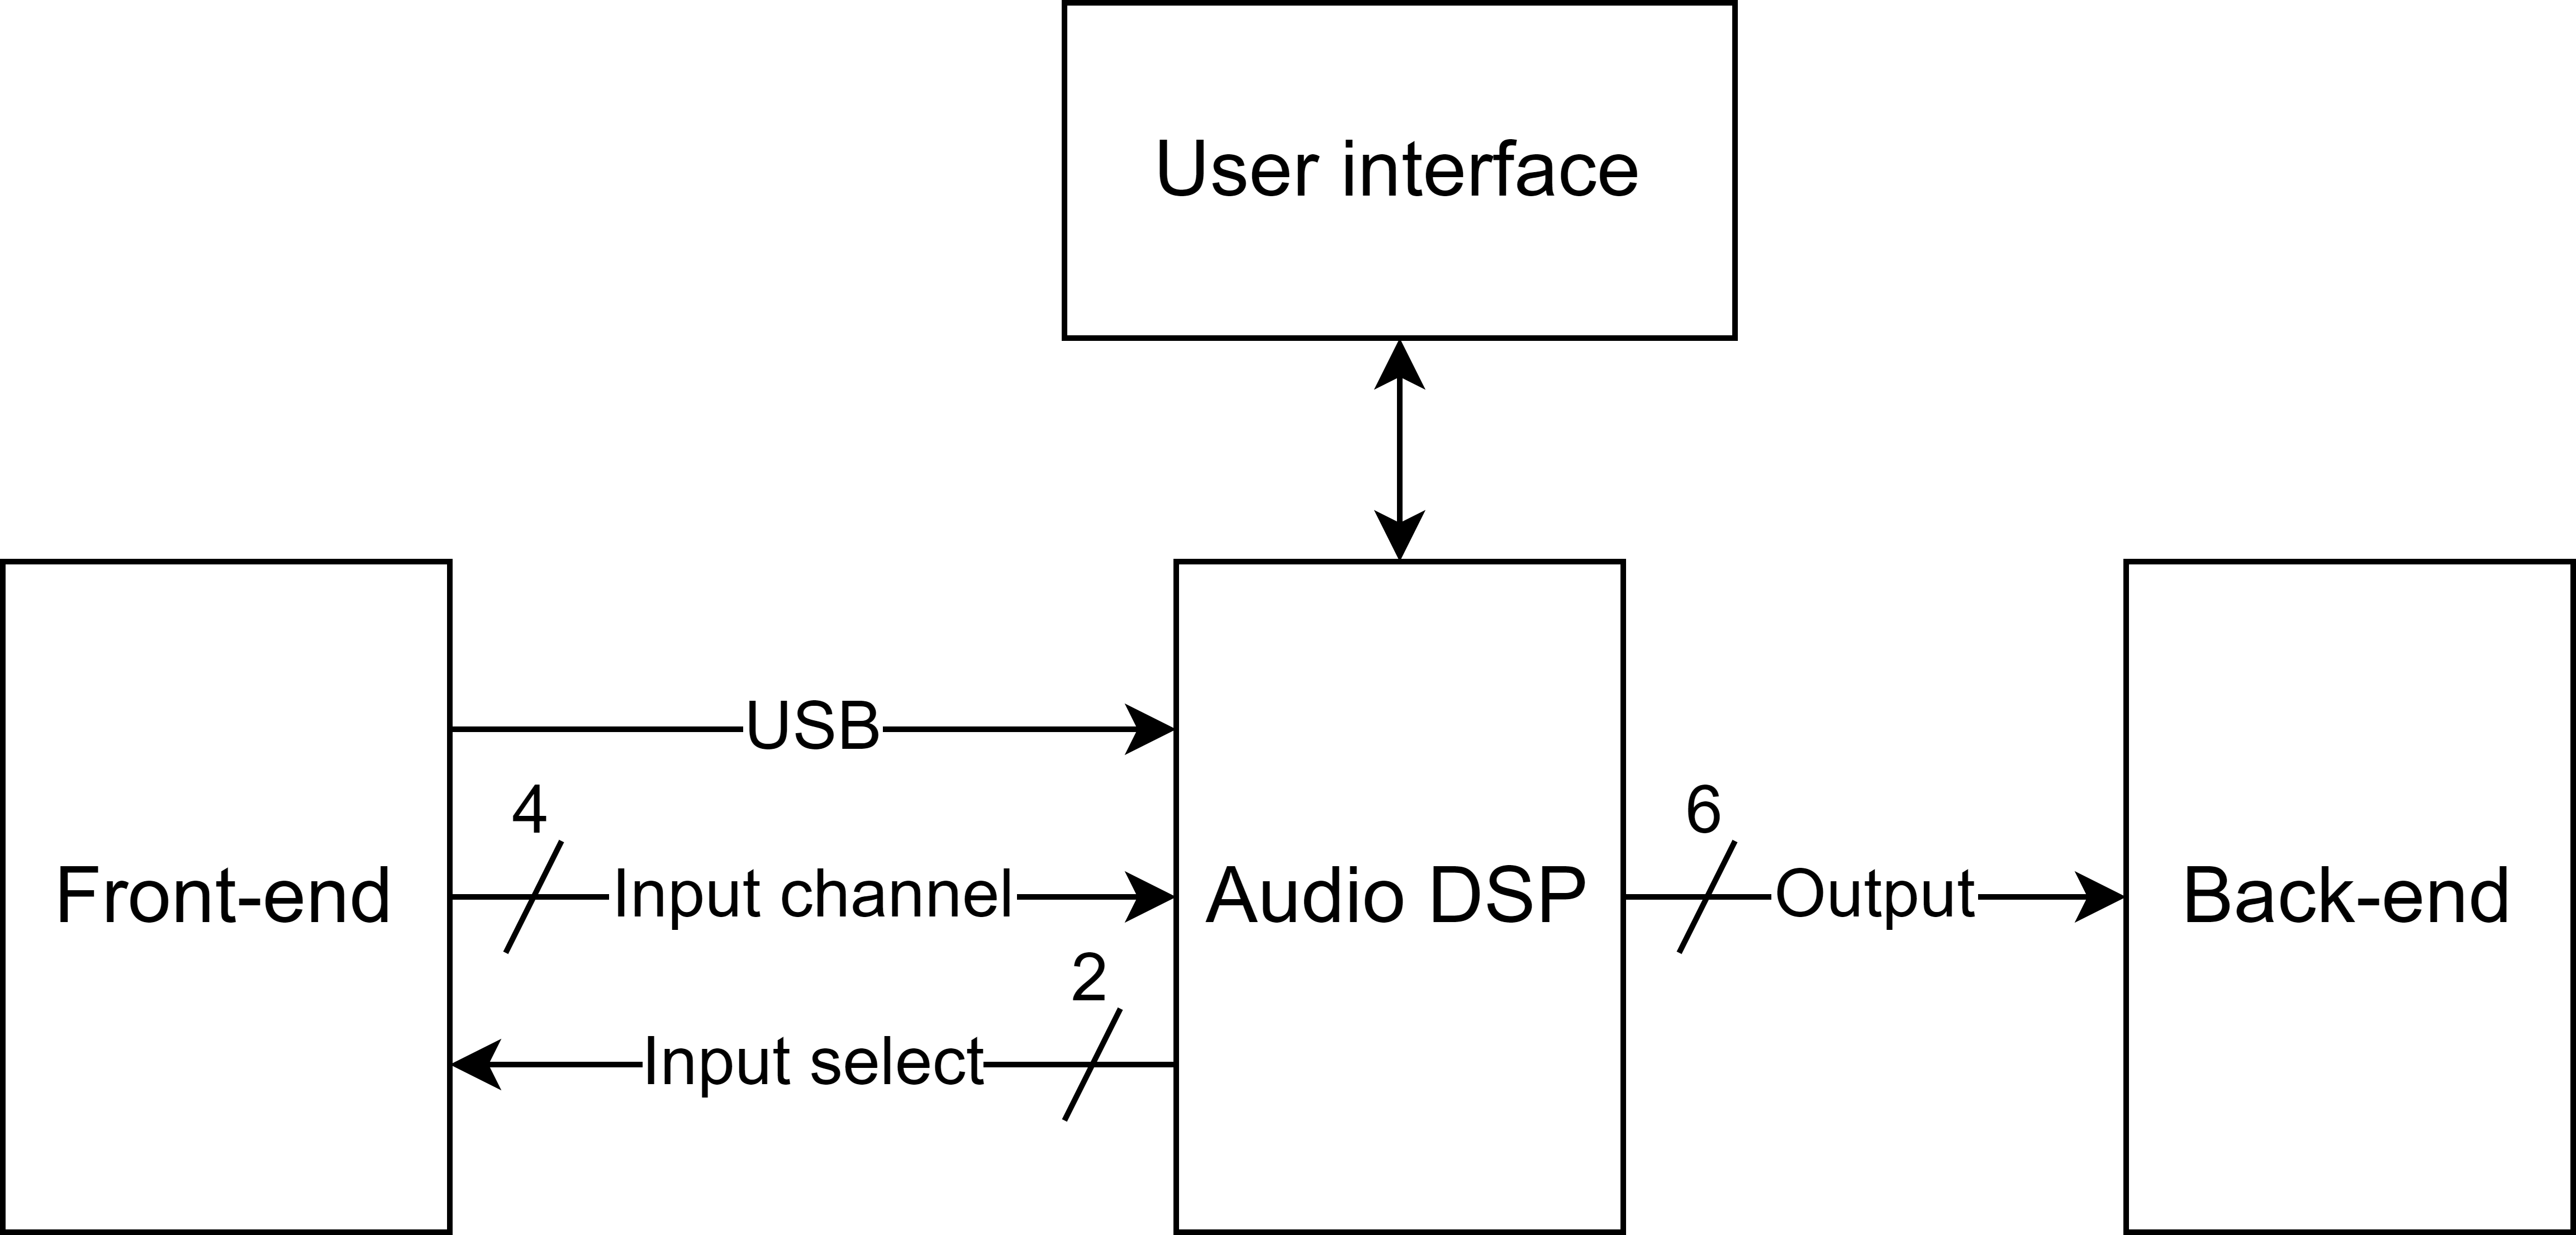
\includegraphics[width=\linewidth]{System context-top level.png}
    \caption{System context diagram of the top-level}
    \label{fig:sys-context-top}
\end{figure}

\section{Front-end}


\begin{figure}[h]
    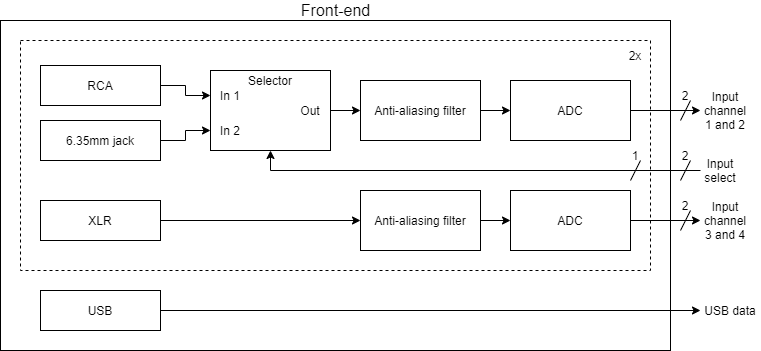
\includegraphics[width=\linewidth]{System context-front-end.png}
    \caption{System context diagram of front-end design}
\end{figure}

\section{Audio-DSP}
\begin{figure}[h]
    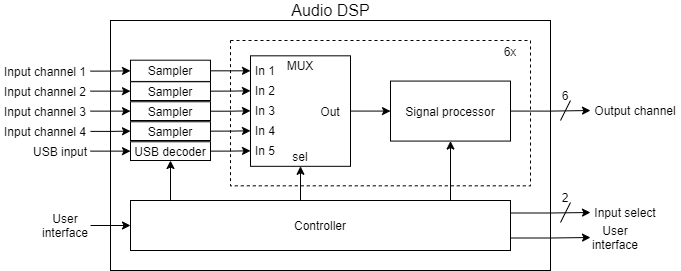
\includegraphics[width=\linewidth]{System context-audio DSP.png}
    \caption{System context diagram of Audio-DSP}
\end{figure}

\section{Back-end}
\begin{figure}[h]
    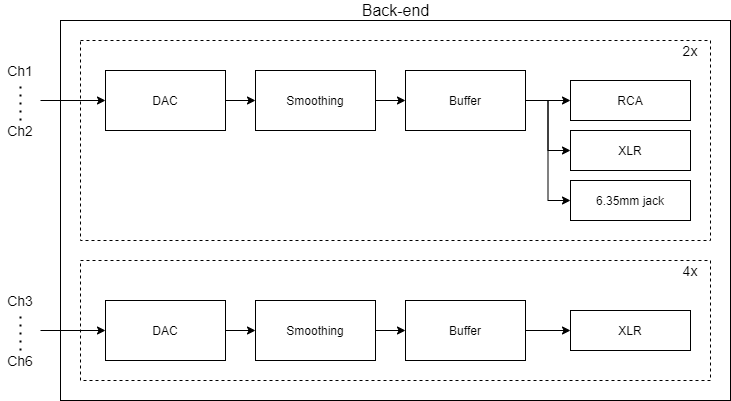
\includegraphics[width=\linewidth]{System context-back-end.png}
    \caption{System context diagram of back-end}
\end{figure}

\section{User interface}
